\documentclass[pt=12]{article}
\usepackage[utf8]{inputenc}
\usepackage{hyperref}


\title{The Deep History of Postwar Global Capitalism}
\author{Julio Huato}
\date{\today}

\usepackage{Sweave}
\begin{document}
\Sconcordance{concordance:test.tex:test.Rnw:%
1 9 1 1 0 17 1 1 2 7 0 1 2 2 1 1 2 5 0 1 2 10 1 1 266 1 2 1 1 1 2 1 0 5 %
1 4 0 1 2 112 1}


\maketitle

\section{Introduction}

The purpose of this article is to grasp the evolving international structure of postwar global capitalism in its empirical complexity, i.e. regarded as a concrete historical totality.

The theoretical framework is explicitly Marxian.  It takes seriously, without hedging, the chief tenets of historical materialism and of the radical critical of political economy from the standpoint of the direct producers of the world.  This radical critique is extended to modern economics.  The tools utilized to extract factual knowledge from the observations compiled in the data set are those of modern, advanced inferential statistics.

The study proceeds in stages progressing from the most simple and general notions, i.e. those based on the most strict and highly abstract premises, to the more complex and specific categories, i.e. those highlighted under more relaxed and concrete hypotheses.  In the earlier stages, the statistical techniques used presuppose that the processes that characterize social life under global capitalism are straightforward.  In the latter stages, these techniques allow for processes that are more involved  However, the progression, as opposed to the mere results, is essential to apprehend the layered nature of the social formation of interest.

This article was typeset with \LaTeX, the data sets were analyzed with $R$, and both data analysis and typesetting were integrated with \texttt{Sweave}.  The $R$ code is inserted in the relevants part of the text in listing form. All the project files are available for public inspection on \textbf{Share}\LaTeX:

\href{https://www.sharelatex.com/project/5724dd4cc9e6d5e323d97763}{\texttt{The Deep History of Postwar Global Capitalism}}


\begin{Schunk}
\begin{Sinput}
> 2+2
\end{Sinput}
\begin{Soutput}
[1] 4
\end{Soutput}
\end{Schunk}

Here I go back to \LaTeX.  And then a curve:

\begin{Schunk}
\begin{Sinput}
> curve(1/x, -2,2, lwd=2, col="violet")
\end{Sinput}
\end{Schunk}
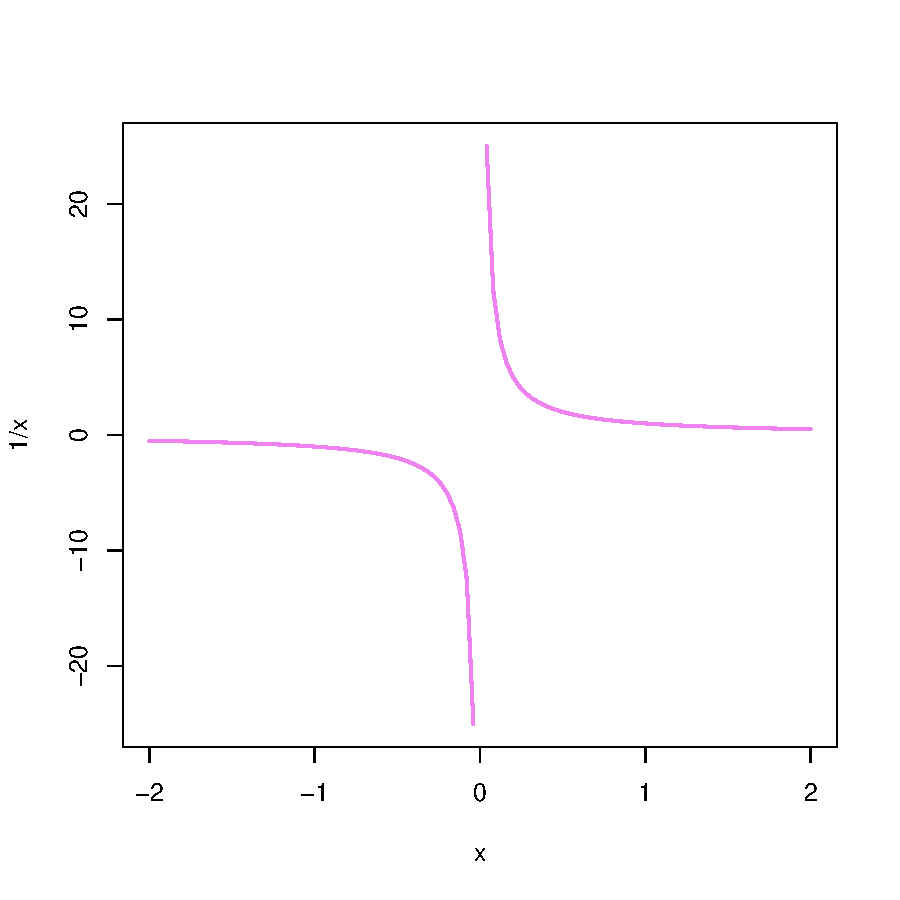
\includegraphics{test-002}

\section{Data}

182 countries, 65 years (1950-2014).  The relevant variables are: $N, E, L, L_h, Y, Y^o, K, W, C$, from which the following variables were derived: 
\[
y_n, y_w, y_l, y_h, k_n, k_w, k_l, k_h, w, c, c^x, c^a, e, \epsilon, \epsilon^x, \epsilon^a, \rho, r, \kappa, \kappa^x, \kappa^a.
\]

\subsection{International unweighted}

Population:
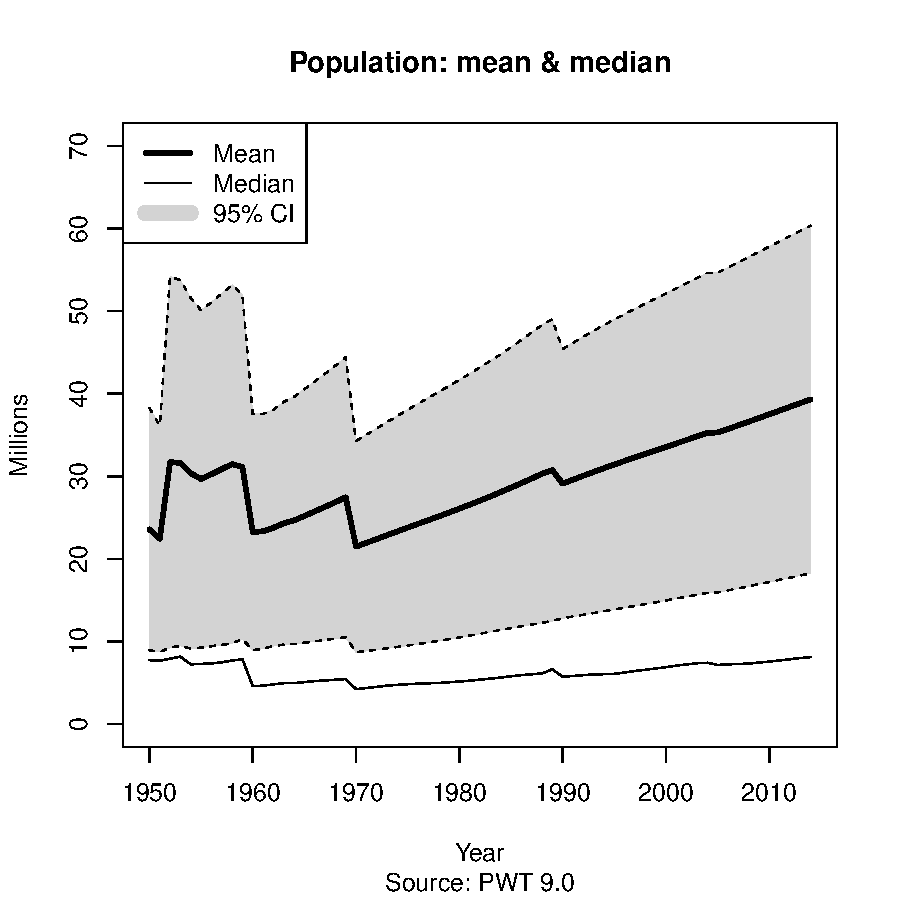
\includegraphics{test-003}

Employment:
\begin{Schunk}
\begin{Sinput}
> plot(descr$year, descr$EMedian, ylim=c(0,30), lwd=1, type="line", main="Employment: mean, median, and 95% CI", ylab="Millions", xlab="Year")
> polygon(x=c(descr$year, rev(descr$year)), y=c(descr$`ELCL Mean`, rev(descr$`EUCL Mean`)), col="lightgray", border=NA)
> lines(descr$year, descr$EMean, col="black", lwd=3)
> lines(descr$year, descr$`ELCL Mean`, col="black", lty=2)
> lines(descr$year, descr$`EUCL Mean`, col="black", lty=2)
> legend("topleft", c("Mean","Median", "95% CI"), lwd=c(3,1,10), lty=c(1,1,1), col=c("black","black", "lightgray"))
\end{Sinput}
\end{Schunk}
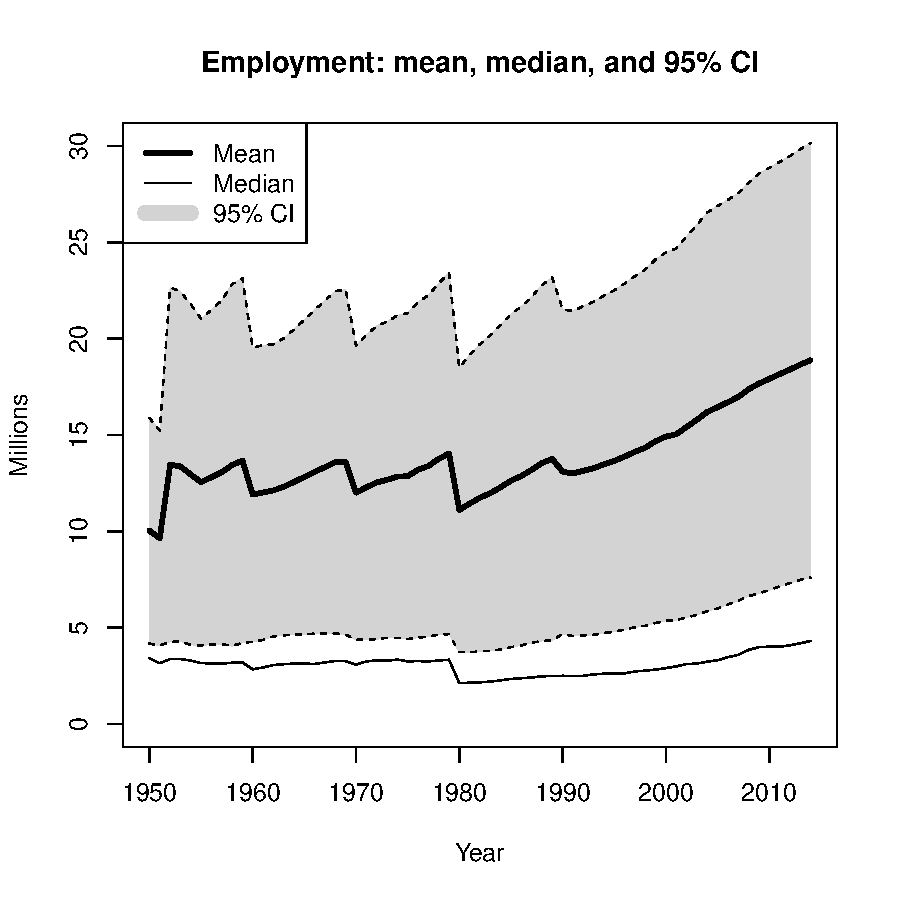
\includegraphics{test-004}



[Include TFP.  How about doing all this at GDP evaluated at average annual exchange rate?]

\section{Theoretical framework}

Historical materialism (relation between productive forces of labor and the social relations of production) and political economy (output as value and as the product of capital, class struggle and competition). 

There are two clearly distinctive ways of interpreting historical materialism:
\begin{enumerate}
\item The productive forces constrain/enable the collective choice of social relations of production.  The social relations of production constrain/enable the collective choice of legal and political systems.  The legal and political system constrain/enable the ideas of people about politics, law, and economics.  Yet, the purposeful actions of individuals change politics, and through them laws, and through them economic structures, and through them technological conditions.  Productive forces, economic structures, and legal/political/ideological superstructure are not different ``things,'' but the same evolving complex society viewed in its different aspects or historical tempos (like anatomy, physiology, and psychology are not different ``things,'' but different aspects of the same evolving human body).
\item Engels argued along these lines in some of his works.  Marx also suggested some of these ideas. People change their ideas because changes in the political, legal, and economic conditions compel them to change their ideas.  This is somewhat plausible: Insofar as you are assuming the absence of socialism, or if you are thinking as something outside of socialism.  The world as it exists in abstraction of socialism.  As a rule, people in our society are atomized, subject to the inertia of existing political, legal, and economic conditions, which are thus because that is what existing productivity allows.

\end{enumerate}

The framework is explicitly Marxian.

The productive forces as developed historically under capitalism can be captured by the following state variables:
\begin{enumerate}
\item $N$: Population
\item $E$: Employment
\item $Y$: Output
\item $K$: Capital stock (wealth controlled by capital)
\end{enumerate}

The following ratios also capture the productive forces under capitalism:
\begin{enumerate}
\item $y \equiv Y/N$: Per-capita output
\item $\bar{y} \equiv Y/E$: Per-worker output
\item $\tilde{y} \equiv Y/L$: Per-hour output
\item $k \equiv K/N$: Per-capita capital
\item $\bar{k} \equiv Y/E$: Per-worker capital
\item $\tilde{y} \equiv Y/L$: Per-hour capital
\item $\rho \equiv Y/K$: Capital effectiveness
\end{enumerate}

The ``economic'' class balance of forces (a summary index of the relations of production) is captured by the following ratios, which are mathematically equivalent:
\begin{enumerate}
\item $\omega \equiv W/Y$: Wage share
\item $\pi \equiv \Pi/Y = 1 - \omega$: Profit share
\item $e \equiv \Pi/W$: Rate of exploitation
\end{enumerate}

Also some measures of unemployment or slack in the economy.  For that, estimate an exponential trend of $Y$ conditional on $N$ (distributed lag model), and fit it on the observed $Y$.  The residuals are a measure of slack in the economy, which increases the political power over the workers.

Another approach: Data from ILO on workers' struggles.  A measure of how combative workers are in a given period of time.  Workers' struggles conditioned on $e$ or $\omega$.

The profit rate summarizes the condition of capital.  It synthesizes two factors: (1) the ``economic'' class balance of forces and (2) the conditions of inter-capitalist competition:
\begin{eqnarray}
r \equiv \frac{\Pi}{K} = \frac{\Pi}{Y} \frac{Y}{K} = \pi \rho, \\
r = \frac{\Pi}{W} \frac{W}{Y} \frac{Y}{K} = e \omega \rho.
\end{eqnarray}

Capital productivity captures the conditions of inter-capitalist competition.

For political conditions, I need to expand the data set.  ILO has a lot on the strength of workers.  Also, one needs to complement that with political parties in office in country $i$ and year $t$.


\section{Global}

Global results and their discussion here.

\section{International (1)}

The results for variables aggregated by population.

\section{International (2)}

The results for variables aggregated by country.

\section{Poor vs. rich}

Here using the classification by high income vs. low income.  Level of capitalist development (use $y$ or $\tilde{y}$ or $\bar{y}$ for that).

\section{Groups}

Using geographic, ethnic, cultural, linguistic classification criteria.  Also, largest ten countries by $Y$ and $N$.

\section{Largest ten countries}

United States, China, Japan, Germany, Brazil, India, etc.  One by one.

Combine here with OECD national accounts and more detailed stats.


\section{Historical evolution}

The methodology used to study the evolution of postwar global capitalism is that of:

\begin{itemize}
\item Time series econometrics
\item Panel econometrics with time effects
\end{itemize}

Time series econometrics follows a successive approximations approach, starting from the most restrictive assumptions (most abstract) to the least restrictive (more concrete and complex).  

First, I take each relevant time series in turn under the assumption of stationarity for ratios and changes in levels and growth rates.  Use of ARMA models.

Second, I assume deterministic trend of relevant levels, and focus on the de-trended series (deviations from the long-run trend). Next stochastic trends.

Third, breaks using Chow and Quandt Likelihood Ratios.

Fourth, I assume relationships among variables: Distributed lag models. 

Fifth, I work on co-integration and VARMA EC modeling.

\begin{eqnarray}
y = 2 x^3
\end{eqnarray}


\end{document}
